\section{Clustering}
\label{sec:clustering}

We compared three clustering algorithms applied to the original
substitute vectors using many-to-one accuracy on the 45-tag 24K word
test corpus.  Hierarchical agglomerative clustering with complete
linkage (HAC) starts with each instance in its own cluster and
iteratively combines the two closest groups (measured by their most
distant points) at each step \cite{manning2008introduction}.
K-medoids minimizes sum of pairwise distances between each datapoint
to the exemplar at the center of its cluster
\cite{kaufman2005finding}.  Spectral clustering\footnote{We used the
  implementation in \cite{chen2011parallel} with a symmetric sparse
  affinity matrix of 550 nearest neighbors.} uses the eigenvalues of
the graph Laplacian $L=D^{-1/2} W D^{-1/2}$ to reduce the number of
dimensions (similar to Laplacian eigenmaps) and uses simple k-means
clustering on the resulting representation \cite{ng2002spectral}.  All
three algorithms accept the distance matrix based on the KL2 distance
(see Section~\ref{sec:dist}) as input.

\begin{figure}[h]
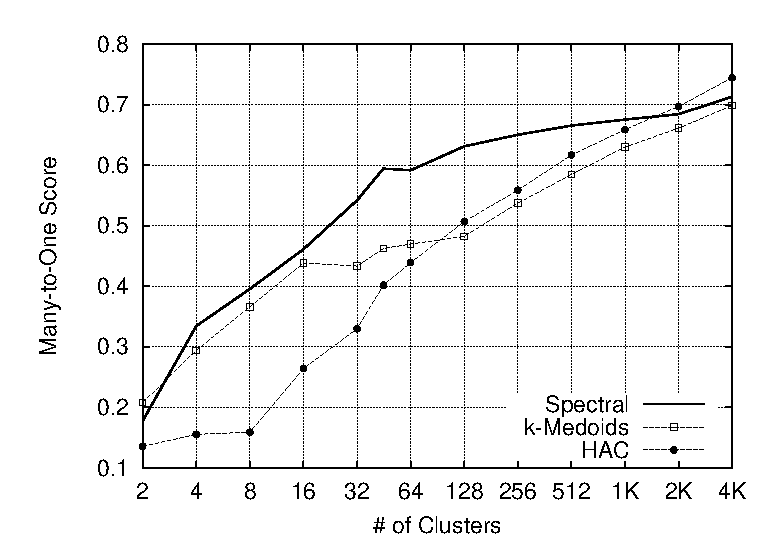
\includegraphics[width=.5\textwidth]{clustering_graph_mono.eps}
\caption{Many-to-one score for three clustering algorithms on the
  45-tag 24K word corpus.}
\label{fig:clustering}
\end{figure}

% #cluster kmedoid spectral hac
% 2          0.20795 0.17781 0.135762
% 4          0.29413 0.33439 0.155579
% 8          0.36615 0.39550 0.159076
% 16        0.43830 0.46116 0.263988
% 32        0.43318 0.54192 0.329850
% 45        0.46245 0.59413 0.401832
% 64        0.46965 0.59151 0.438843
% 128      0.48235 0.63106 0.506703
% 256      0.53709 0.65000 0.558659
% 512      0.58464 0.66520 0.616653
% 1024     0.62985 0.67523 0.658576
% 2048     0.66107 0.68414 0.696878
% 4096     0.69842 0.71286 0.744338


Figure~\ref{fig:clustering} plots the many-to-one score versus number
of clusters for the three algorithms on the 45-tag 24K word test
corpus.  The many-to-one score naturally increases as we approach the
one cluster per word limit, however we find the evolution of the
curves informative.  At the high end (more than 2000 clusters) HAC
performs best with its conservative clusters, but its performance
degrades fast as we reduce the number of clusters because it cannot
reverse the accumulating mistakes.  At the low end (less than 16
clusters) k-medoids and spectral have similar performance.  However
for the region of interest (between 16 to 2000 clusters) spectral
clustering is clearly superior with \spectralResult\% many-to-one
accuracy at 45 clusters.

